\chapter{Suunnatut verkot}

Tämä luku käsittelee kahta suunnattuihin
verkkoihin liittyvää aihetta.
Ensin keskitymme verkkoihin, joissa ei ole silmukoita.
Tämä mahdollistaa topologisen järjestyksen
muodostamisen verkon solmuille,
minkä ansiosta verkossa voi edelleen
käyttää dynaamista ohjelmointia.

Tämän jälkeen tutustumme funktionaalisiin
verkkoihin eli verkkoihin, joissa jokaisesta solmusta
lähtee tasan yksi kaari.
Tällaisessa verkossa jokaisella solmulla on
yksikäsitteinen seuraaja ja verkossa etenemiseen
ja syklien etsimiseen on olemassa tehokkaita algoritmeja.

\section{Topologinen järjestys}

Topologinen järjestys
(\textit{topological sort}) on tapa
järjestää suunnatun verkon solmut niin,
että jos solmusta $a$ pääsee solmuun $b$,
niin $a$ on ennen $b$:tä järjestyksessä.
Esimerkiksi jos solmut ovat kursseja
ja kaaret ovat kurssien esitietovaatimukset,
topologinen järjestys antaa
tavan suorittaa kaikki kurssit.

Esimerkiksi verkon
\begin{center}
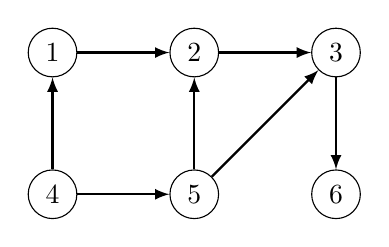
\begin{tikzpicture}[scale=0.9]
\node[draw, circle] (1) at (1,5) {$1$};
\node[draw, circle] (2) at (3,5) {$2$};
\node[draw, circle] (3) at (5,5) {$3$};
\node[draw, circle] (4) at (1,3) {$4$};
\node[draw, circle] (5) at (3,3) {$5$};
\node[draw, circle] (6) at (5,3) {$6$};

\path[draw,thick,->,>=latex] (1) -- (2);
\path[draw,thick,->,>=latex] (2) -- (3);
\path[draw,thick,->,>=latex] (4) -- (1);
\path[draw,thick,->,>=latex] (4) -- (5);
\path[draw,thick,->,>=latex] (5) -- (2);
\path[draw,thick,->,>=latex] (5) -- (3);
\path[draw,thick,->,>=latex] (3) -- (6);
\end{tikzpicture}
\end{center}

yksi topologinen järjestys on
$(4, 1, 5, 2, 3, 6)$:
\begin{center}
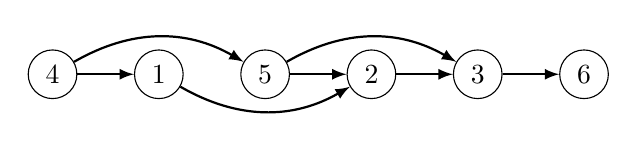
\begin{tikzpicture}[scale=0.9]
\node[draw, circle] (1) at (-6,0) {$1$};
\node[draw, circle] (2) at (-3,0) {$2$};
\node[draw, circle] (3) at (-1.5,0) {$3$};
\node[draw, circle] (4) at (-7.5,0) {$4$};
\node[draw, circle] (5) at (-4.5,0) {$5$};
\node[draw, circle] (6) at (-0,0) {$6$};

\path[draw,thick,->,>=latex] (1) edge [bend right=30] (2);
\path[draw,thick,->,>=latex] (2) -- (3);
\path[draw,thick,->,>=latex] (4) -- (1);
\path[draw,thick,->,>=latex] (4) edge [bend left=30] (5);
\path[draw,thick,->,>=latex] (5) -- (2);
\path[draw,thick,->,>=latex] (5) edge [bend left=30]  (3);
\path[draw,thick,->,>=latex] (3) -- (6);
\end{tikzpicture}
\end{center}

Topologinen järjestys on olemassa
aina silloin, kun verkossa ei ole sykliä.
Jos taas verkossa on sykli,
topologista järjestystä ei voi muodostaa.
Seuraavaksi näemme, miten syvyyshaun avulla
voi muodostaa topologisen järjestyksen tai
todeta, että tämä ei ole mahdollista syklin takia.

\subsubsection{Algoritmi}

Ideana on käydä läpi verkon solmut syvyyshaulla,
jossa on kolme tilaa:

\begin{itemize}
\item tila 0: solmua ei ole käsitelty (valkoinen)
\item tila 1: solmun käsittely on alkanut (vaaleanharmaa)
\item tila 2: solmu on käsitelty (tummanharmaa)
\end{itemize}

Aluksi jokaisen verkon solmun tila on 0.
Kun syvyyshaku saapuu solmuun, sen tilaksi tulee 1.
Lopuksi kun syvyyshaku on käsitellyt kaikki
solmun naapurit, solmun tilaksi tulee 2.

Jos verkossa on sykli, tämä selviää syvyyshaun aikana siitä,
että jossain vaiheessa haku saapuu solmuun,
jonka tila on 1. Tässä tapauksessa topologista
järjestystä ei voi muodostaa.

Jos verkossa ei ole sykliä, topologinen järjestys
saadaan muodostamalla lista, johon kukin solmu lisätään
silloin, kun sen tilaksi tulee 2.
Tämä lista käänteisenä on yksi verkon
topologinen järjestys.

\subsubsection{Esimerkki 1}

Esimerkkiverkossa syvyyshaku etenee ensin solmusta 1
solmuun 6 asti:

\begin{center}
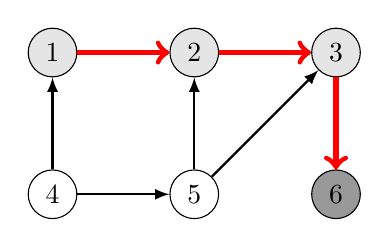
\begin{tikzpicture}[scale=0.9]
\node[draw, circle,fill=gray!20] (1) at (1,5) {$1$};
\node[draw, circle,fill=gray!20] (2) at (3,5) {$2$};
\node[draw, circle,fill=gray!20] (3) at (5,5) {$3$};
\node[draw, circle] (4) at (1,3) {$4$};
\node[draw, circle] (5) at (3,3) {$5$};
\node[draw, circle,fill=gray!80] (6) at (5,3) {$6$};

%\path[draw,thick,->,>=latex] (1) -- (2);
%\path[draw,thick,->,>=latex] (2) -- (3);
\path[draw,thick,->,>=latex] (4) -- (1);
\path[draw,thick,->,>=latex] (4) -- (5);
\path[draw,thick,->,>=latex] (5) -- (2);
\path[draw,thick,->,>=latex] (5) -- (3);
%\path[draw,thick,->,>=latex] (3) -- (6);

\path[draw=red,thick,->,line width=2pt] (1) -- (2);
\path[draw=red,thick,->,line width=2pt] (2) -- (3);
\path[draw=red,thick,->,line width=2pt] (3) -- (6);
\end{tikzpicture}
\end{center}

Tässä vaiheessa solmu 6 on käsitelty, joten se lisätään listalle.
Sen jälkeen haku palaa takaisinpäin:

\begin{center}
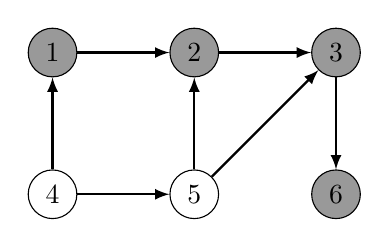
\begin{tikzpicture}[scale=0.9]
\node[draw, circle,fill=gray!80] (1) at (1,5) {$1$};
\node[draw, circle,fill=gray!80] (2) at (3,5) {$2$};
\node[draw, circle,fill=gray!80] (3) at (5,5) {$3$};
\node[draw, circle] (4) at (1,3) {$4$};
\node[draw, circle] (5) at (3,3) {$5$};
\node[draw, circle,fill=gray!80] (6) at (5,3) {$6$};

\path[draw,thick,->,>=latex] (1) -- (2);
\path[draw,thick,->,>=latex] (2) -- (3);
\path[draw,thick,->,>=latex] (4) -- (1);
\path[draw,thick,->,>=latex] (4) -- (5);
\path[draw,thick,->,>=latex] (5) -- (2);
\path[draw,thick,->,>=latex] (5) -- (3);
\path[draw,thick,->,>=latex] (3) -- (6);
\end{tikzpicture}
\end{center}

Tämän jälkeen listan sisältönä on $(6,3,2,1)$.
Seuraavaksi syvyyshaun toinen vaihe alkaa solmusta 4:

\begin{center}
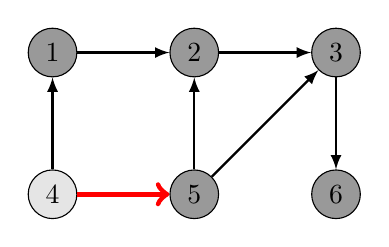
\begin{tikzpicture}[scale=0.9]
\node[draw, circle,fill=gray!80] (1) at (1,5) {$1$};
\node[draw, circle,fill=gray!80] (2) at (3,5) {$2$};
\node[draw, circle,fill=gray!80] (3) at (5,5) {$3$};
\node[draw, circle,fill=gray!20] (4) at (1,3) {$4$};
\node[draw, circle,fill=gray!80] (5) at (3,3) {$5$};
\node[draw, circle,fill=gray!80] (6) at (5,3) {$6$};

\path[draw,thick,->,>=latex] (1) -- (2);
\path[draw,thick,->,>=latex] (2) -- (3);
\path[draw,thick,->,>=latex] (4) -- (1);
%\path[draw,thick,->,>=latex] (4) -- (5);
\path[draw,thick,->,>=latex] (5) -- (2);
\path[draw,thick,->,>=latex] (5) -- (3);
\path[draw,thick,->,>=latex] (3) -- (6);

\path[draw=red,thick,->,line width=2pt] (4) -- (5);
\end{tikzpicture}
\end{center}

Tämän seurauksena listaksi tulee $(6,3,2,1,5,4)$.
Kaikki solmut on käyty läpi, joten topologinen järjestys on valmis.
Se on lista käänteisenä eli $(4,5,1,2,3,6)$:

\begin{center}
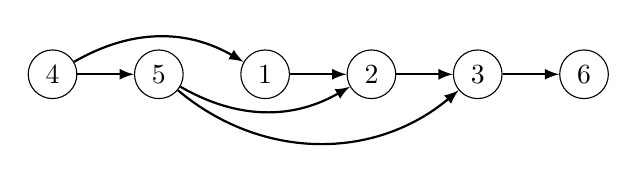
\begin{tikzpicture}[scale=0.9]
\node[draw, circle] (1) at (3,0) {$1$};
\node[draw, circle] (2) at (4.5,0) {$2$};
\node[draw, circle] (3) at (6,0) {$3$};
\node[draw, circle] (4) at (0,0) {$4$};
\node[draw, circle] (5) at (1.5,0) {$5$};
\node[draw, circle] (6) at (7.5,0) {$6$};

\path[draw,thick,->,>=latex] (1) -- (2);
\path[draw,thick,->,>=latex] (2) -- (3);
\path[draw,thick,->,>=latex] (4) edge [bend left=30] (1);
\path[draw,thick,->,>=latex] (4) -- (5);
\path[draw,thick,->,>=latex] (5) edge [bend right=30] (2);
\path[draw,thick,->,>=latex] (5) edge [bend right=40] (3);
\path[draw,thick,->,>=latex] (3) -- (6);
\end{tikzpicture}
\end{center}

Huomaa, että topologinen järjestys ei ole yksikäsitteinen,
vaan verkolla voi olla useita topologisia järjestyksiä.

\subsubsection{Esimerkki 2}

Tarkastellaan sitten tilannetta, jossa topologista järjestystä
ei voi muodostaa syklin takia. Näin on seuraavassa verkossa:

\begin{center}
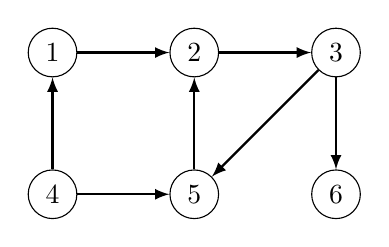
\begin{tikzpicture}[scale=0.9]
\node[draw, circle] (1) at (1,5) {$1$};
\node[draw, circle] (2) at (3,5) {$2$};
\node[draw, circle] (3) at (5,5) {$3$};
\node[draw, circle] (4) at (1,3) {$4$};
\node[draw, circle] (5) at (3,3) {$5$};
\node[draw, circle] (6) at (5,3) {$6$};

\path[draw,thick,->,>=latex] (1) -- (2);
\path[draw,thick,->,>=latex] (2) -- (3);
\path[draw,thick,->,>=latex] (4) -- (1);
\path[draw,thick,->,>=latex] (4) -- (5);
\path[draw,thick,->,>=latex] (5) -- (2);
\path[draw,thick,->,>=latex] (3) -- (5);
\path[draw,thick,->,>=latex] (3) -- (6);
\end{tikzpicture}
\end{center}

Nyt syvyyshaun aikana tapahtuu näin:

\begin{center}
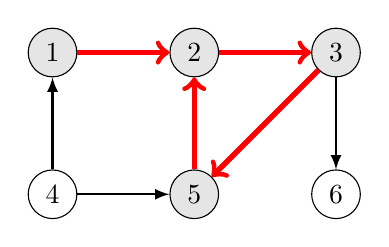
\begin{tikzpicture}[scale=0.9]
\node[draw, circle,fill=gray!20] (1) at (1,5) {$1$};
\node[draw, circle,fill=gray!20] (2) at (3,5) {$2$};
\node[draw, circle,fill=gray!20] (3) at (5,5) {$3$};
\node[draw, circle] (4) at (1,3) {$4$};
\node[draw, circle,fill=gray!20] (5) at (3,3) {$5$};
\node[draw, circle] (6) at (5,3) {$6$};

%\path[draw,thick,->,>=latex] (1) -- (2);
%\path[draw,thick,->,>=latex] (2) -- (3);
\path[draw,thick,->,>=latex] (4) -- (1);
\path[draw,thick,->,>=latex] (4) -- (5);
%\path[draw,thick,->,>=latex] (5) -- (2);
%\path[draw,thick,->,>=latex] (3) -- (5);
\path[draw,thick,->,>=latex] (3) -- (6);

\path[draw=red,thick,->,line width=2pt] (1) -- (2);
\path[draw=red,thick,->,line width=2pt] (2) -- (3);
\path[draw=red,thick,->,line width=2pt] (3) -- (5);
\path[draw=red,thick,->,line width=2pt] (5) -- (2);
\end{tikzpicture}
\end{center}

Syvyyshaku saapuu tilassa 1 olevaan solmuun 2,
mikä tarkoittaa, että verkossa on sykli.
Tässä tapauksessa sykli on $2 \rightarrow 3 \rightarrow 5 \rightarrow 2$.

\section{Dynaaminen ohjelmointi}

Jos suunnatussa verkossa ei ole sykliä, sen solmuihin voi
soveltaa dynaamista ohjelmointia topologisessa järjestyksessä.
Dynaamisen ohjelmoinnin avulla voi vastata esimerkiksi seuraaviin
kysymyksiin koskien verkossa olevia polkuja solmusta $a$ solmuun $b$:

\begin{itemize}
\item montako erilaista polkua on olemassa?
\item mikä on pienin/suurin mahdollinen määrä kaaria polulla?
\item mitkä solmut esiintyvät varmasti polulla?
\end{itemize}

Tutustumme seuraavaksi tekniikkaan käyttäen
esimerkkinä polkujen määrän laskemista verkossa.

\subsection{Polkujen määrä}

\begin{task}
Annettuna on suunnattu verkko, jossa ei ole sykliä.
Tehtäväsi on laskea, montako polkua on olemassa
solmusta $a$ solmuun $b$.
\end{task}

\begin{samepage}
Esimerkiksi verkossa

\begin{center}
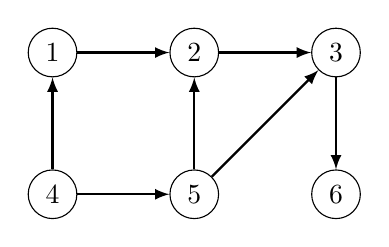
\begin{tikzpicture}[scale=0.9]
\node[draw, circle] (1) at (1,5) {$1$};
\node[draw, circle] (2) at (3,5) {$2$};
\node[draw, circle] (3) at (5,5) {$3$};
\node[draw, circle] (4) at (1,3) {$4$};
\node[draw, circle] (5) at (3,3) {$5$};
\node[draw, circle] (6) at (5,3) {$6$};

\path[draw,thick,->,>=latex] (1) -- (2);
\path[draw,thick,->,>=latex] (2) -- (3);
\path[draw,thick,->,>=latex] (4) -- (1);
\path[draw,thick,->,>=latex] (4) -- (5);
\path[draw,thick,->,>=latex] (5) -- (2);
\path[draw,thick,->,>=latex] (5) -- (3);
\path[draw,thick,->,>=latex] (3) -- (6);
\end{tikzpicture}
\end{center}
\end{samepage}

on 3 polkua solmusta 4 solmuun 6:

\begin{itemize}
\item $4 \rightarrow 1 \rightarrow 2 \rightarrow 3 \rightarrow 6$
\item $4 \rightarrow 5 \rightarrow 2 \rightarrow 3 \rightarrow 6$
\item $4 \rightarrow 5 \rightarrow 3 \rightarrow 6$
\end{itemize}

Ideana on käydä läpi verkon solmut topologisessa järjestyksessä
ja laskea kunkin solmun kohdalla yhteen eri suunnista
tulevien polkujen määrät.
Verkon topologinen järjestys on seuraava:

\begin{center}
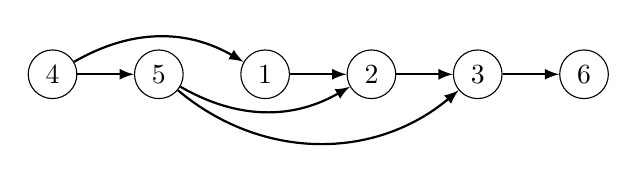
\begin{tikzpicture}[scale=0.9]
\node[draw, circle] (1) at (3,0) {$1$};
\node[draw, circle] (2) at (4.5,0) {$2$};
\node[draw, circle] (3) at (6,0) {$3$};
\node[draw, circle] (4) at (0,0) {$4$};
\node[draw, circle] (5) at (1.5,0) {$5$};
\node[draw, circle] (6) at (7.5,0) {$6$};

\path[draw,thick,->,>=latex] (1) -- (2);
\path[draw,thick,->,>=latex] (2) -- (3);
\path[draw,thick,->,>=latex] (4) edge [bend left=30] (1);
\path[draw,thick,->,>=latex] (4) -- (5);
\path[draw,thick,->,>=latex] (5) edge [bend right=30] (2);
\path[draw,thick,->,>=latex] (5) edge [bend right=40] (3);
\path[draw,thick,->,>=latex] (3) -- (6);
\end{tikzpicture}
\end{center}

Tuloksena ovat seuraavat lukumäärät:

\begin{center}
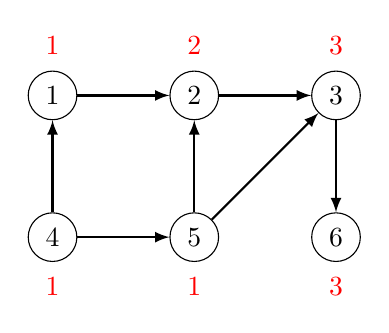
\begin{tikzpicture}[scale=0.9]
\node[draw, circle] (1) at (1,5) {$1$};
\node[draw, circle] (2) at (3,5) {$2$};
\node[draw, circle] (3) at (5,5) {$3$};
\node[draw, circle] (4) at (1,3) {$4$};
\node[draw, circle] (5) at (3,3) {$5$};
\node[draw, circle] (6) at (5,3) {$6$};

\path[draw,thick,->,>=latex] (1) -- (2);
\path[draw,thick,->,>=latex] (2) -- (3);
\path[draw,thick,->,>=latex] (4) -- (1);
\path[draw,thick,->,>=latex] (4) -- (5);
\path[draw,thick,->,>=latex] (5) -- (2);
\path[draw,thick,->,>=latex] (5) -- (3);
\path[draw,thick,->,>=latex] (3) -- (6);

\node[color=red] at (1,2.3) {$1$};
\node[color=red] at (3,2.3) {$1$};
\node[color=red] at (5,2.3) {$3$};
\node[color=red] at (1,5.7) {$1$};
\node[color=red] at (3,5.7) {$2$};
\node[color=red] at (5,5.7) {$3$};
\end{tikzpicture}
\end{center}

Esimerkiksi solmuun 2 pääsee solmuista 1 ja 5.
Kumpaankin solmuun päättyy yksi polku solmusta 4 alkaen,
joten solmuun 2 päättyy kaksi polkua solmusta 4 alkaen.
Vastaavasti solmuun 3 pääsee solmuista 2 ja 5,
joiden kautta tulee kaksi ja yksi polkua solmusta 4 alkaen.

\subsection{Dijkstran sovellukset}

Dijkstran algoritmin sivutuotteena syntyy suunnattu, syklitön verkko,
joka kertoo jokaiselle alkuperäisen verkon solmulle,
mitä tapoja alkusolmusta on päästä kyseiseen solmuun lyhintä
polkua käyttäen.
Tähän verkkoon voi soveltaa edelleen dynaamista ohjelmointia.

Esimerkiksi verkossa
\begin{center}
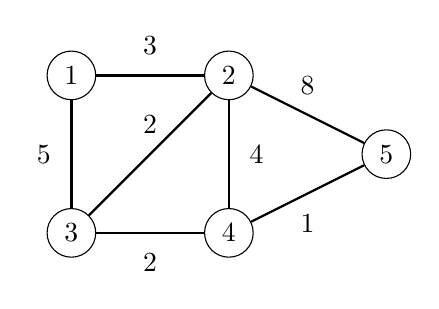
\begin{tikzpicture}
\node[draw, circle] (1) at (0,0) {$1$};
\node[draw, circle] (2) at (2,0) {$2$};
\node[draw, circle] (3) at (0,-2) {$3$};
\node[draw, circle] (4) at (2,-2) {$4$};
\node[draw, circle] (5) at (4,-1) {$5$};

\path[draw,thick,-] (1) -- node[font=\small,label=above:3] {} (2);
\path[draw,thick,-] (1) -- node[font=\small,label=left:5] {} (3);
\path[draw,thick,-] (2) -- node[font=\small,label=right:4] {} (4);
\path[draw,thick,-] (2) -- node[font=\small,label=above:8] {} (5);
\path[draw,thick,-] (3) -- node[font=\small,label=below:2] {} (4);
\path[draw,thick,-] (4) -- node[font=\small,label=below:1] {} (5);
\path[draw,thick,-] (2) -- node[font=\small,label=above:2] {} (3);
\end{tikzpicture}
\end{center}

solmusta 1 lähteviin lyhimpiin polkuihin kuuluvat
seuraavat kaaret:
\begin{center}
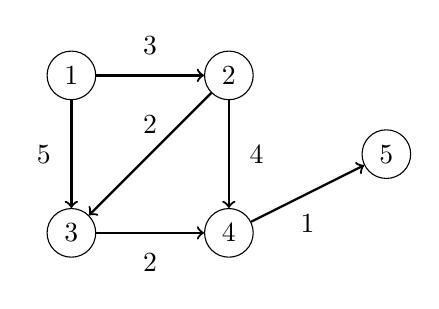
\begin{tikzpicture}
\node[draw, circle] (1) at (0,0) {$1$};
\node[draw, circle] (2) at (2,0) {$2$};
\node[draw, circle] (3) at (0,-2) {$3$};
\node[draw, circle] (4) at (2,-2) {$4$};
\node[draw, circle] (5) at (4,-1) {$5$};

\path[draw,thick,->] (1) -- node[font=\small,label=above:3] {} (2);
\path[draw,thick,->] (1) -- node[font=\small,label=left:5] {} (3);
\path[draw,thick,->] (2) -- node[font=\small,label=right:4] {} (4);
\path[draw,thick,->] (3) -- node[font=\small,label=below:2] {} (4);
\path[draw,thick,->] (4) -- node[font=\small,label=below:1] {} (5);
\path[draw,thick,->] (2) -- node[font=\small,label=above:2] {} (3);
\end{tikzpicture}
\end{center}

Koska kyseessä on suunnaton, syklitön verkko,
siihen voi soveltaa dynaamista ohjelmointia.
Niinpä voi esimerkiksi laskea, montako lyhintä polkua
on olemassa solmusta 1 solmuun 5:
\begin{center}
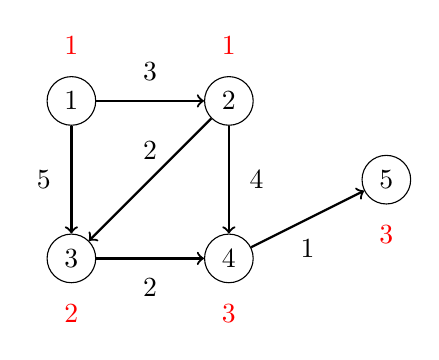
\begin{tikzpicture}
\node[draw, circle] (1) at (0,0) {$1$};
\node[draw, circle] (2) at (2,0) {$2$};
\node[draw, circle] (3) at (0,-2) {$3$};
\node[draw, circle] (4) at (2,-2) {$4$};
\node[draw, circle] (5) at (4,-1) {$5$};

\path[draw,thick,->] (1) -- node[font=\small,label=above:3] {} (2);
\path[draw,thick,->] (1) -- node[font=\small,label=left:5] {} (3);
\path[draw,thick,->] (2) -- node[font=\small,label=right:4] {} (4);
\path[draw,thick,->] (3) -- node[font=\small,label=below:2] {} (4);
\path[draw,thick,->] (4) -- node[font=\small,label=below:1] {} (5);
\path[draw,thick,->] (2) -- node[font=\small,label=above:2] {} (3);

\node[color=red] at (0,0.7) {$1$};
\node[color=red] at (2,0.7) {$1$};
\node[color=red] at (0,-2.7) {$2$};
\node[color=red] at (2,-2.7) {$3$};
\node[color=red] at (4,-1.7) {$3$};
\end{tikzpicture}
\end{center}


\section{Funktionaaliset verkot}

Funktionaalinen verkko (\textit{functional graph})
on suunnattu verkko, jonka jokaisesta solmusta lähtee
tasan yksi kaari ulospäin.
Funktionaalinen verkko muodostuu yhdestä tai
useammasta komponentista, joista jokaisessa
on yksi sykli ja joukko siihen johtavia polkuja.

Termi ''funktionaalinen'' johtuu siitä,
että jokaista funktionaalista verkkoa vastaa
funktio $f$, joka määrittelee verkon kaaret.
Funktion parametrina on verkon solmu ja
se palauttaa solmusta lähtevän kaaren kohdesolmun.
Verkon kaaret ovat siis muotoa $(x,f(x))$,
missä $s=1,2,\ldots,n$.

\begin{samepage}
Esimerkiksi funktio

\begin{center}
\begin{tabular}{r|rrrrrrrrr}
$x$ & 1 & 2 & 3 & 4 & 5 & 6 & 7 & 8 & 9 \\
\hline
$f(x)$ & 3 & 5 & 7 & 6 & 2 & 2 & 1 & 6 & 3 \\
\end{tabular}
\end{center}
\end{samepage}

määrittelee seuraavan verkon:

\begin{center}
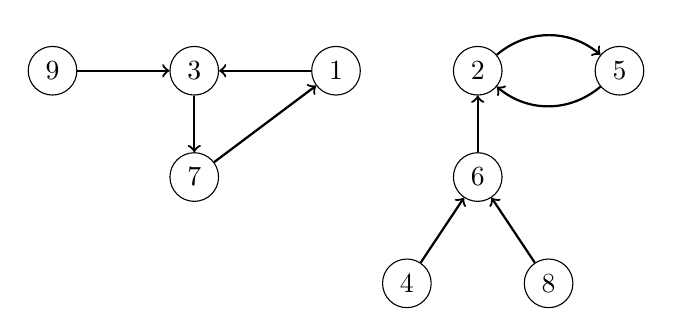
\begin{tikzpicture}[scale=0.9]
\node[draw, circle] (1) at (0,0) {$1$};
\node[draw, circle] (2) at (2,0) {$2$};
\node[draw, circle] (3) at (-2,0) {$3$};
\node[draw, circle] (4) at (1,-3) {$4$};
\node[draw, circle] (5) at (4,0) {$5$};
\node[draw, circle] (6) at (2,-1.5) {$6$};
\node[draw, circle] (7) at (-2,-1.5) {$7$};
\node[draw, circle] (8) at (3,-3) {$8$};
\node[draw, circle] (9) at (-4,0) {$9$};

\path[draw,thick,->] (1) -- (3);
\path[draw,thick,->] (2)  edge [bend left=40] (5);
\path[draw,thick,->] (3) -- (7);
\path[draw,thick,->] (4) -- (6);
\path[draw,thick,->] (5)  edge [bend left=40] (2);
\path[draw,thick,->] (6) -- (2);
\path[draw,thick,->] (7) -- (1);
\path[draw,thick,->] (8) -- (6);
\path[draw,thick,->] (9) -- (3);
\end{tikzpicture}
\end{center}

\subsection{Nopea eteneminen}

Koska funktionaalisessa verkossa jokaisella solmulla
on yksikäsitteinen seuraaja, voimme määritellä funktion $f(x,k)$,
joka kertoo solmun, johon päätyy solmusta $x$
kulkemalla $k$ askelta.
Esimerkiksi yllä olevassa verkossa $f(4,6)=2$,
koska solmusta 4 päätyy solmuun 2 kulkemalla 6 askelta:

\begin{center}
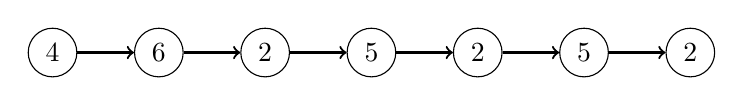
\begin{tikzpicture}[scale=0.9]
\node[draw, circle] (1) at (0,0) {$4$};
\node[draw, circle] (2) at (1.5,0) {$6$};
\node[draw, circle] (3) at (3,0) {$2$};
\node[draw, circle] (4) at (4.5,0) {$5$};
\node[draw, circle] (5) at (6,0) {$2$};
\node[draw, circle] (6) at (7.5,0) {$5$};
\node[draw, circle] (7) at (9,0) {$2$};

\path[draw,thick,->] (1) -- (2);
\path[draw,thick,->] (2) -- (3);
\path[draw,thick,->] (3) -- (4);
\path[draw,thick,->] (4) -- (5);
\path[draw,thick,->] (5) -- (6);
\path[draw,thick,->] (6) -- (7);
\end{tikzpicture}
\end{center}

Suoraviivainen tapa laskea funktion $f(x,k)$ arvo
on käydä läpi polku verkossa askel askeleelta, mihin kuluu aikaa $O(k)$.
Sopivan esikäsittelyn avulla kuitenkin minkä tahansa
funktion arvon pystyy laskemaan ajassa $O(\log k)$.

Ideana on laskea etukäteen funktion $f(x,k)$ arvot, kun $k$ on 2:n potenssi.
Tämä onnistuu tehokkaasti, koska $f(x,1)=f(x)$ ja $f(x,k)=f(f(x,k/2),k/2)$.
Esilaskenta vie aikaa $O(n \log k)$, koska jokaisesta solmusta
lasketaan $O(\log k)$ arvoa.
Esimerkin tapauksessa muodostuu seuraava taulukko:

\begin{center}
\begin{tabular}{r|rrrrrrrrr}
$x$ & 1 & 2 & 3 & 4 & 5 & 6 & 7 & 8 & 9 \\
\hline
$f(x,1)$ & 3 & 5 & 7 & 6 & 2 & 2 & 1 & 6 & 3 \\
$f(x,2)$ & 7 & 2 & 1 & 2 & 5 & 5 & 3 & 2 & 7 \\
$f(x,4)$ & 3 & 2 & 7 & 2 & 5 & 5 & 1 & 2 & 3 \\
$f(x,8)$ & 7 & 2 & 1 & 2 & 5 & 5 & 3 & 2 & 7 \\
$\cdots$ \\
\end{tabular}
\end{center}

Tämän jälkeen funktion $f(x,k)$ arvon saa laskettua
esittämällä luvun $k$ summana 2:n potensseja.
Esimerkiksi $11=8+2+1$, joten $f(x,11)=f(f(f(x,8),2),1)$.
Niinpä yllä olevassa verkossa 
$f(4,11)=f(f(f(4,8),2),1)=5$.
Polussa on aina $O(\log k)$ osaa, joten laskemiseen
kuluu aikaa $O(\log k)$.

\subsection{Syklin etsiminen}

Toinen kiinnostava kysymys funktionaalisessa verkossa on,
kuinka monta askelta solmusta $x$ tulee kulkea
ennen sykliin pääsemistä ja mikä on syklin pituus.
Esimerkiksi yllä olevassa verkossa solmusta 9
pääsee sykliin kulkemalla yhden askeleen
ja sykliin kuuluu kolme solmua (1, 3 ja 7).

Helppo tapa etsiä sykli on alkaa kulkea verkossa
solmusta $x$ alkaen ja pitää kirjaa kaikista vastaan tulevista
solmuista. Kun jokin solmu tulee vastaan toista kertaa,
sykli on löytynyt. Tämän menetelmän aikavaativuus on $O(n)$
ja muistia kuluu myös $O(n)$.

Osoittautuu kuitenkin, että ongelman ratkaisuun on
olemassa parempia algoritmeja.
Niissä aikavaativuus on edelleen $O(n)$,
mutta muistia kuluu vain $O(1)$.
Tästä on merkittävää hyötyä, jos $n$ on suuri.
Tutustumme seuraavaksi kahteen tällaiseen algoritmiin.

\subsubsection{Algoritmi 1 (Floyd)}

Floydin algoritmi kulkee verkossa eteenpäin rinnakkain
kahdesta kohdasta.
Osoitin $a$ liikkuu joka vuorolla askeleen eteenpäin,
kun taas osoitin $b$ liikkuu kaksi askelta eteenpäin.
Haku jatkuu, kunnes osoittimet kohtaavat:

\begin{lstlisting}
a = f(x);
b = f(f(x));
while (a != b) {
    a = f(a);
    b = f(f(b));
}
\end{lstlisting}

Tässä vaiheessa osoitin $a$ on kulkenut $k$ askelta
ja osoitin $b$ on kulkenut $2k$ askelta,
missä $k$ on jaollinen syklin pituudella.
Niinpä ensimmäinen sykliin kuuluva solmu löytyy siirtämällä
osoitin $a$ alkuun ja liikuttamalla osoittimia
rinnakkain eteenpäin, kunnes ne kohtaavat.

\begin{lstlisting}
a = x;
while (a != b) {
    a = f(a);
    b = f(b);
}
\end{lstlisting}

Nyt $a$ ja $b$ osoittavat ensimmäiseen syklin
solmuun, joka tulee vastaan solmusta $x$ lähdettäessä.
Lopuksi syklin pituus $c$ voidaan laskea näin:

\begin{lstlisting}
b = f(a);
c = 1;
while (a != b) {
    b = f(b);
    c++;
}
\end{lstlisting}

\subsubsection{Algoritmi 2 (Brent)}

Brentin algoritmi
muodostuu peräkkäisistä vaiheista, joissa osoitin $a$ pysyy
paikallaan ja osoitin $b$ liikkuu $k$ askelta
Alussa $k=1$ ja $k$:n arvo kaksinkertaistuu
joka vaiheen alussa.
Lisäksi $a$ siirretään $b$:n kohdalle vaiheen alussa.
Näin jatketaan, kunnes osoittimet kohtaavat.

\begin{lstlisting}
a = x;
b = f(x);
c = k = 1;
while (a != b) {
    if (c == k) {
        a = b;
        c = 0;
        k *= 2;
    }
    b = f(b);
    c++;
}
\end{lstlisting}

Nyt tiedossa on, että syklin pituus on $c$.
Tämän jälkeen ensimmäinen sykliin kuuluva solmu löytyy
palauttamalla ensin osoittimet alkuun,
siirtämällä sitten osoitinta $b$ eteenpäin $c$ askelta
ja liikuttamalla lopuksi osoittimia rinnakkain,
kunnes ne osoittavat samaan solmuun.

\begin{lstlisting}
a = b = x;
for (int i = 0; i < c; i++) b = f(b);
while (a != b) {
    a = f(a);
    b = f(b);
}
\end{lstlisting}

Nyt $a$ ja $b$ osoittavat ensimmäiseen sykliin kuuluvaan solmuun.

Brentin algoritmin etuna Floydin algoritmiin verrattuna on,
että se kutsuu funktiota $f$ harvemmin.
Floydin algoritmi kutsuu funktiota $f$ ensimmäisessä silmukassa
kolmesti joka kierroksella, kun taas Brentin algoritmi
kutsuu funktiota $f$ vain kerran kierrosta kohden.